\subsection{Decomposition}
	The compilation dependencies are as follows:
	\begin{itemize}
		\item Android dependencies a user will have an array of visits
		\item A visit will have an array of specimens
		\item A specimen can get data from the plant db (Fig \ref{fig:androidComponentDiagram}).
	\end{itemize}
	
	\begin{figure}
		\centering
			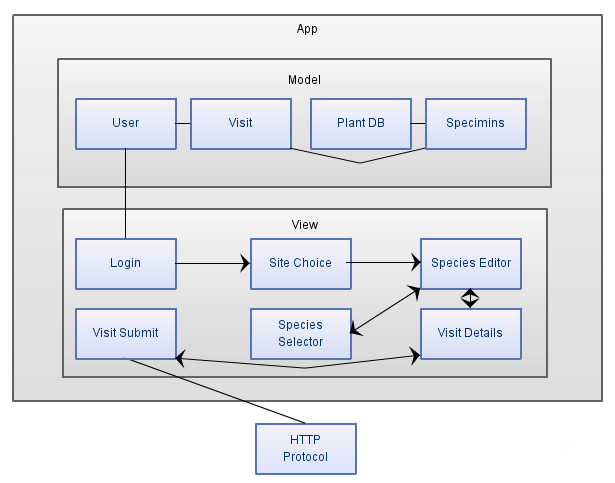
\includegraphics[scale=0.75]{android/componentDiagram.png}
		\caption{Component diagram for Android}
		\label{fig:androidComponentDiagram}
	\end{figure}

\newpage
\subsection{Interfaces}
	\subsubsection{Login Activity Interface}
		\lstinputlisting[language=Java, firstline=33]{android/src/loginInterface.java}

	\newpage
	\subsubsection{Site Choice Activity Interface}
		\lstinputlisting[language=Java, firstline=8]{android/src/siteChoiceInterface.java}

	\newpage
	\subsubsection{Species Selector Activity Interface}
		\lstinputlisting[language=Java, firstline=8]{android/src/speciesSelectorInterface.java}

	\newpage
	\subsubsection{Visit Management Activity Interface}
		\lstinputlisting[language=Java, firstline=8]{android/src/visitManagementInterface.java}

	\newpage
	\subsubsection{Visit Submit Activity Interface}
		\lstinputlisting[language=Java, firstline=8]{android/src/visitSubmitInterface.java}

	\newpage
	\subsubsection{User Data Class Interface}
		\lstinputlisting[language=Java, firstline=1]{android/src/userClassInterface.java}

	\newpage
	\subsubsection{Visit Data Class Interface}
		\lstinputlisting[language=Java, firstline=1]{android/src/visitClassInterface.java}

	\newpage
	\subsubsection{Plant DB Interface}
		This Will be a file obtained from the Botanical Society of Britain and Ireland containing a large list of known plant types in a comma sperated list (CSV) format. This file will be parsed at runtime and a condensed list created in alphabetical order for searching. Obtained from $http://www.bsbi.org.uk/resources.html$

	\subsubsection{Specimen Class Interface}
		\lstinputlisting[language=Java, firstline=1]{android/src/SpecimenClassInterface.java}
